\documentclass[11pt, oneside]{article}   	% use "amsart" instead of "article" for AMSLaTeX format
\usepackage{geometry}                		% See geometry.pdf to learn the layout options. There are lots.
\geometry{letterpaper}                   		% ... or a4paper or a5paper or ... 
%\geometry{landscape}                		% Activate for rotated page geometry
%\usepackage[parfill]{parskip}    		% Activate to begin paragraphs with an empty line rather than an indent
\usepackage{graphicx}				% Use pdf, png, jpg, or eps§ with pdflatex; use eps in DVI mode
								% TeX will automatically convert eps --> pdf in pdflatex		
\usepackage{amssymb}
\usepackage{amsmath}
\usepackage[colorlinks, urlcolor=blue, linkcolor=black]{hyperref}
\usepackage{listings}
\usepackage{xcolor}
\usepackage{float}
\lstset { %
    language=C++,
    backgroundcolor=\color{white}, % set backgroundcolor
    basicstyle=\footnotesize,% basic font setting
}

%SetFonts

%SetFonts


\title{FYS 4150 Project 1 Report}
\author{Marc Kidwell Pestana}
\date{}							% Activate to display a given date or no date

\begin{document}
\maketitle
\section{Abstract}
The aim of this project is to get familiar with various vector and matrix operations, from dynamic memory allocation to the usage of programs in the library package of the course.
\section{Introduction}
This is a report written by myself for Project1, Computation Physics 2017. A copy of this report as well as C++ programming code, and other related files can be found at:\newline\newline
\href{https://github.com/marckp/project1}{project1 master branch}\newline
\href{https://github.com/marckp/project1/tree/master/project1}{C++ code}\newline
\href{https://github.com/marckp/project1/tree/master/project1/Documentation}{Project 1 report and results}
\section{Software Design, Theoretical Models, and Algorithms}
\subsection{Software Design}
The following list contains a brief description of software implementation practices and guidelines for how I design, code, and test software programs.
\begin{itemize}
\item I use a simple software development cycle: documentation $\leftrightarrow$ coding. I general begin, as I describe next, with documentation. However, there is no requirement here. The process is simple, I alternate between documenting my code and writing my code. I find that process improves both the quality of the programs and their documents.
\item How I start: l lay the groundwork for my software programs by writing down in my own words, what I want the program to accomplish and how the program will accomplish it. This forms the basis for what are commonly referred to as functional requirements. In the case of Project 1, I focused mainly on understanding the mathematical development of the algorithm. In the case of Project 1,  I started by getting a clear understanding the functional requirements by understanding the recursion equations involved with Gaussian Elimination using forward and backward substitutions. I was unable to complete the LU decomposition part of the project.
\item Up front development: do the hard part first. This can mean either getting a clear understanding of the most central and most complicated parts of the program written into the documentation, building the data source needed by the program to function,  writing test programs, or any other development that's needed before the program can function or be tested properly.
\item Regression testing: after each program upgrade, verify that the new program reproduces the same results when appropriate. As described below, two algorithms were tested, the first dealing with the estimation of the second derivative and the associated tri-diagonal matrix, and the second dealing with a generalization of this system to one that is still tri-diagonal, but doesn't restrict the values of the diagonal elements to -1, 2, and 1.
\end{itemize}
In the case of Project 1, navigating the class repository and class documentation to be the most challenging, followed by establishing the development platform, overcoming my resistence to using C++ in which I have no fluency, and understanding the details of the algorithm. That is the order in which I approached project 1. \newline
With respect to the development of the C++ code for Project 1:
\begin{itemize}
\item Project 1 code base was started from a listing I found in the lecture material under the heading "Project 1 hints". 
\item Project 1 requires two input parameters determining the number of steps to be used by the algorithm in it's approximation  to the solution of the the one-dimensional Poisson equation with Dirichlet boundary conditions. I decided to have the program read the input parameters from the command line. Also, I used this parameter to build the input matrix to the algorithm.
\item Project 1 requires the input of tri-diagonal vectors elements. In all cases I have hardcoded the inputs so that they meet the requirements of the algorithms.
\end{itemize} Two functions were developed in which  one was a generalization of the others. Tests were performed to verify the each function gave identical results when setup with identical inputs.
\subsection{Theoretical Models for Project 1}
\subsubsection{Project 1a}
In this project we will solve the one-dimensional Poisson equation with Dirichlet boundary conditions by rewriting it as a set of linear equations.
To be more explicit we will solve the equation:\newline
\newline
$-u^{\prime\prime} (x)=f(x)$, $x \in (0,1), u(0) = u(1) = 1$\newline
\newline
and we define the discretized approximation to $u$ as $v_i$ with grid points $x_i=ih$ in the interval from $x_0=0$ to $x_{n+1}=1$. The step length or spacing is defined as $h=\frac{1}{(n+1)}$. We have then the boundary conditions $v_0=v_{n+1}=0$. We approximate the second derivative of $u$ with\newline
\newline
$-(v_{i+1} + v_{i-1} - 2v_i)/{h^2} = f_i$ for $i = 1,...,n$,\newline
\newline
where $f_i=f(x_i)$.\newline
These equations can be re-written as a set of n linear equations in n unknows by distributing the $-1$ and multiplying both sides by $h^2$ and rearranging the terms, which gives\newline
\newline
$-v_{i-1} + 2v_i  - v_{i+1}=h^2 f_i$ for $i = 1,...,n$,\newline
\newline
Expanding these equations and applying the boundary conditions yields\newline
\newline
\begin{align*}
2v_1 - v_2 &= h^2 f_1 \\
-v_1 + 2v_2 - v_3 &= h^2f_2\\
-v_2 + 2v_3 - v_4 &= h^3f_2\\.\\.\\.\\
-v_{n-1} + 2v_n &= h^3f_n
\end{align*}\newline
\newline
Letting $\vec{v}$ the vector of unknowns as follows\newline
\newline
$\vec{v}=  \begin{bmatrix}
v_1\\
v_2\\
.\\
.\\
v_n
\end{bmatrix}$\newline
\newline
Letting $\vec{b}$ the vector of values for $h^2f(x)$ evaluated at each $x_i$ as follows\newline
\newline
$\vec{b}=  \begin{bmatrix}
b_1\\
b_2\\
.\\
.\\
b_n
\end{bmatrix}  =   \begin{bmatrix}
h^2f(x_1)\\
h^2f(x_2)\\
.\\
.\\
h^2f(x_n)
\end{bmatrix}$\newline
\newline
So the following matrix equation holds
\newline
\newline
$\begin{bmatrix}
2 & -1 & ..& ..& ..& ..& ..& ..\\
-1 & 2 & -1 & .. & ..& ..& ..& ..\\
.. & .. & ..& ..& ..& ..& ..& ..\\
.. & .. & .. & .. & .. & -1 & 2 & -1\\
.. & .. & .. & .. & .. & .. & -1 & 2
\end{bmatrix}  \begin{bmatrix}
v_1\\
v_2\\
.\\
.\\
v_n
\end{bmatrix} =  \begin{bmatrix}
h^2f(x_1)\\
h^2f(x_2)\\
.\\
.\\
h^2f(x_n)
\end{bmatrix}$\newline
\newline\newline
$\quad Let \quad \hat{A} = \begin{bmatrix}
2 & -1 & ..& ..& ..& ..& ..& ..\\
-1 & 2 & -1 & .. & ..& ..& ..& ..\\
.. & .. & ..& ..& ..& ..& ..& ..\\
.. & .. & .. & .. & .. & -1 & 2 & -1\\
.. & .. & .. & .. & .. & .. & -1 & 2
\end{bmatrix}\quad then$,\newline
\newline
$ \hat{A}\vec{v} = \vec{b}$\newline
\newline
\subsubsection{Project 1b}
I will now develop an algorithm to solve a generalization of the "tridiagonal" system introduced in section 1a. A tridiagonal matrix is a special form of banded matrix where all the elements are zero except for those on and immediately above and below the leading diagonal. The above tridiagonal system can be generalized into the following system:\newline
\newline 
$a_iu_{i-1}+d_iu_i+c_iu_{i+1}=f_i\quad i=1,...,n$\newline
\newline
for $i=1,2,...,n$. We see that $u_0$ and $u_{n+1}$ are 0 (boundary conditions) and not required and we can set $a_1=c_n=0$. So  the lower diagonal elements $a_i$, the diagonal elements $d_i$, and the upper diagonal elements $c_i$ give $\hat{A}$ the general form:\newline
\newline
$\quad Let \quad \hat{A} = \begin{bmatrix}
d_1 & c_1 & ..& ..& ..& ..& ..& ..\\
a_2 & d_2 & c_2 & .. & ..& ..& ..& ..\\
.. & a_3 & d_3 & c_3 & .. & .. & .. & ..\\
.. & .. & .. & .. & .. & .. & .. & ..\\
.. & .. & .. & .. & .. & a_{n-1} & d_{n-1} & c_{n-1}\\
.. & .. & .. & .. & .. & .. & a_n & d_n
\end{bmatrix}\quad then$,\newline
\newline
In order that Gaussian Elimination is guaranteed to yield a solution to the tridiagonal system the elements of $\hat{A}$ must satisfy two conditions: 1) elements of $\hat{A}$ statisfy the following relations:
\newline
$|b_1|>|c_1|$, and, $|b_n|>|a_n|$, and, $|b_n| \le |a_n|+|c_n|$\newline
This is called the dominance condition. 2) If the off diagonal elements are non-zero, that is the $a_i$ and $c_i$ are non-zero so that $\hat{A}$ is irreducible. If these two conditions are present, the $\hat{A}$ is nonsingular and has a unique LU decomposition, and so the linear system that $\hat{A}$ represents has a unique solution.\newline
\newline
I began the Gaussian Elimination with putting $\hat{A}$ into the proper form for backward substitution (starting with the last row), by performing a forward substitution (elimination starting with the first row). The desired form is to have only non-zero upper diagonal and diagonal elements. Since the first row of $\hat{A}$ is already in the proper form, the first step in the algorithm begins with a modification to the second row using the first row. The $i^{th}$ step modifies the ${i+1}^{th}$ row using the $i^{th}$ row for a total of $n-1$ modifications. So the general algorithm is defined inductively as follows:\newline
\newline
$i^{th}$ step: subtract $a_{i+1}a_i/\tilde{d_i}$ times the updated $i^{th}$ row from the ${i+1}^{th}$ row as illustrated\newline
\newline
Before:\newline
\newline
$\begin{bmatrix}
0 & \tilde{d_i} & c_i & ..& ..& ..& ..& ..& ..\\
0 & a_{i+1} & d_{i+1} & c_{i+1} & .. & ..& ..& ..& ..
\end{bmatrix}$\newline
\newline
After:\newline
\newline
$\begin{bmatrix}
0 & \tilde{d_i} & c_i & 0 & 0 & ..& ..& ..& ..\\
0 & 0 & d_{i+1} - a_{i+1}c_i/\tilde{d_i} & c_{i+1} & 0 & ..& ..& ..& ..
\end{bmatrix}$\newline
\newline
So that the ${i+1}^{th}$ row becomes:\newline
\newline
$\begin{bmatrix}
0 & \tilde{d_i} & c_i & 0 & 0 & ..& ..& ..& ..\\
0 & 0 & \tilde{d}_{i+1} & c_{i+1} & 0 & ..& ..& ..& ..
\end{bmatrix}$\newline
\newline
where $\tilde{d}_{i+1} = d_{i+1} - a_{i+1}c_i/\tilde{d_i}$ \newline
\newline
Since we are solving the general linear system above, the same steps are applied to both sides of $\hat{A}\vec{u} = \vec{f}$, so that\newline
\newline
$\tilde{f}_{i+1} = f_{i+1} - a_{i+1}\tilde{f}_i/\tilde{d_i}$\newline
\newline
Now I can employ backward substitution to find the solution $\vec{u}$. Starting with the last row, solve for $u_n$ which gives:\newline
\newline
$u_n = \tilde{f}_n/\tilde{d}_n$\newline
\newline
starting from the solution from the $i^{th}$  row to  ${i-1}^{th}$ row, solve for $u_{i-1}$ as follows:\newline
\newline
$u_{i-1}=(\tilde{f}_i -c_{i-1}u_i)/\tilde{d}_{i-1}$\newline
\newline
\section{Results and discussion}
The program I created takes two command line inputs: root name of the file into which a table of results were stored, and the second is the highest exponent of 10 used to determine the step size increment. So executing the following command would perform the tri-diagonal elimination method using step sizes of 10, 100, 1000, 10000, 100000, and 1000000. This command also created 6 files with the stem 'test' appending  the step size exponent to the stem resulting in the creation of test1, test2, test3, test4, test5, and test6. 
prompt>./project1 test 6<return>

Two functions were defined using C++ forward declaration techniques:\newline
// C++ code\newline
void simpleTridiagonalAlg(int n,double *sol,double *x);\newline
void generalTridiagonalAlg(int n,double *u,double *x,double *d,double *c,double *a);\newline
// end C++ code\newline

As shown, the arrays used for the 3 diagonals of the system were created using dynamic memory allocation. Regression testing was performed to verify that the two functions agreed when the function for the general case was supplied  with the values for the a[i]'s, d[i]'s, and c[i]'s corresponding to the system described in part 1 a), i.e. a[i] = -1, d[i] =2, and c[i] = -1. Testing was perform by running the program twice using first the simple form of the algorithm and then with the generalized form. The files from the first run were compared with the output files of the second run using the LINUX diff command that reports any ascii differences between two files on a line by line basis. Both functions produced identical results.

\begin{figure}[H]
  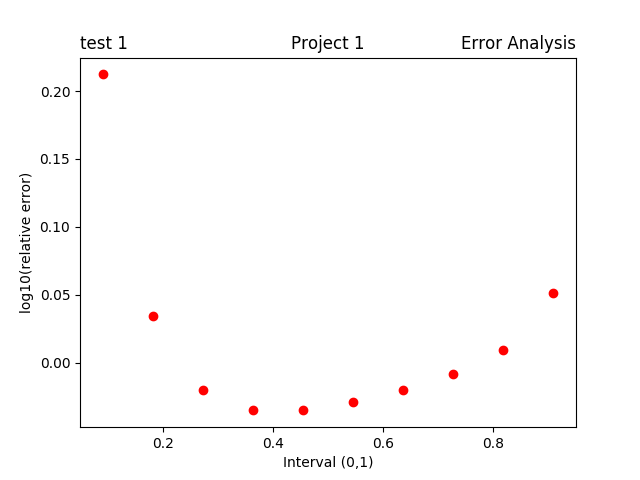
\includegraphics[width=\linewidth]{test_1.png}
  \caption{Step size of $10^{-1}$}
  \label{fig:Relative Error}
\end{figure}

\begin{figure}[H]
  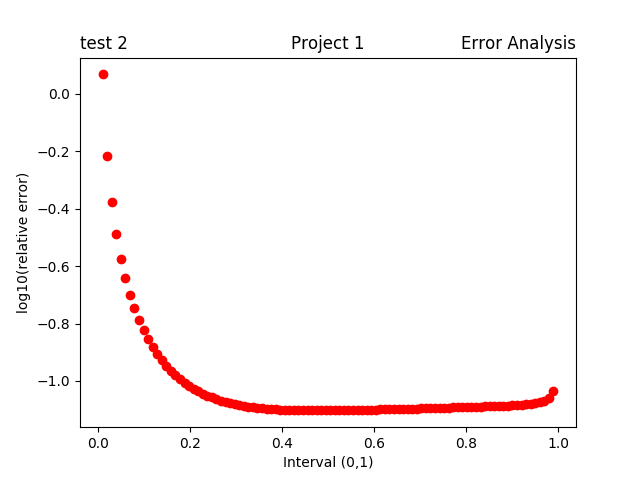
\includegraphics[width=\linewidth]{test_2.png}
  \caption{Step size of $10^{-2}$}
  \label{fig:boat1}
\end{figure}

\begin{figure}[H]
  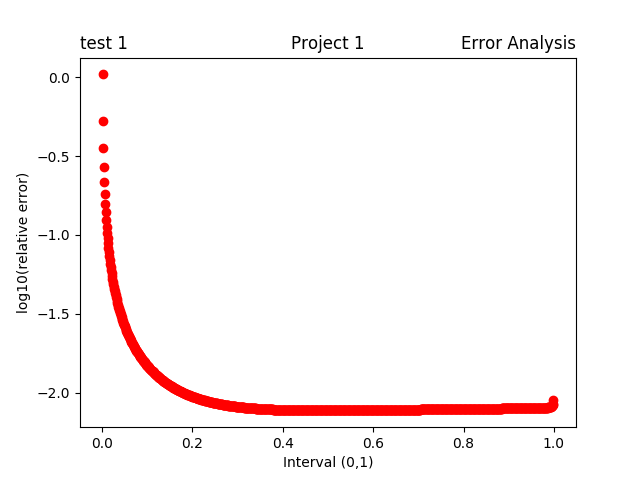
\includegraphics[width=\linewidth]{test_3.png}
  \caption{Step size of $10^{-3}$}
  \label{fig:Relative Error}
\end{figure}

 \begin{figure}[H]
  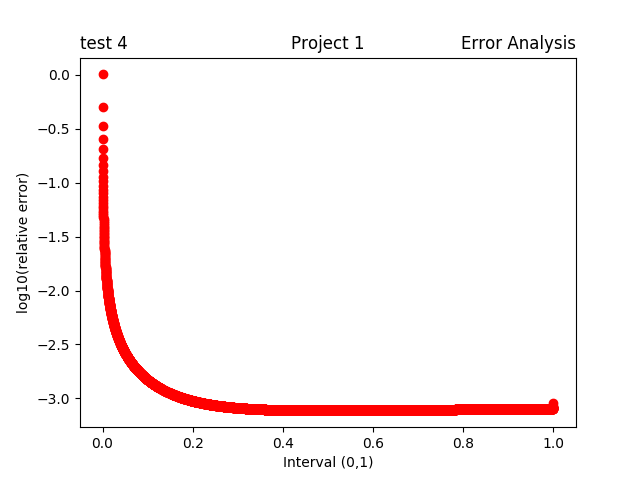
\includegraphics[width=\linewidth]{test_4.png}
  \caption{Step size of $10^{-4}$}
  \label{fig:Relative Error}
\end{figure}

\begin{figure}[H]
  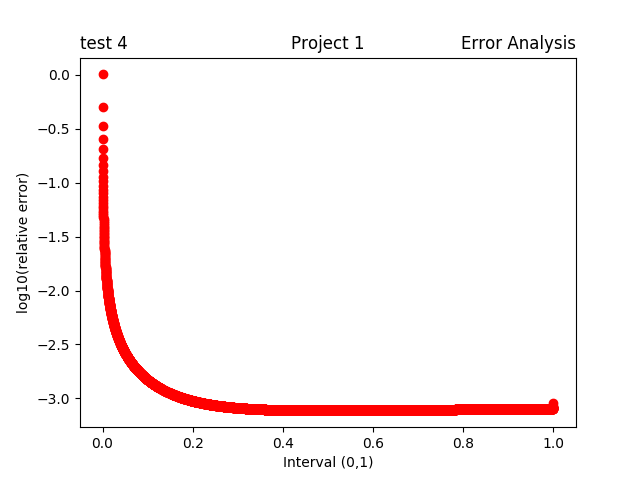
\includegraphics[width=\linewidth]{test_5.png}
  \caption{Step size of $10^{-5}$}
  \label{fig:Relative Error}
\end{figure}

\begin{figure}[H]
  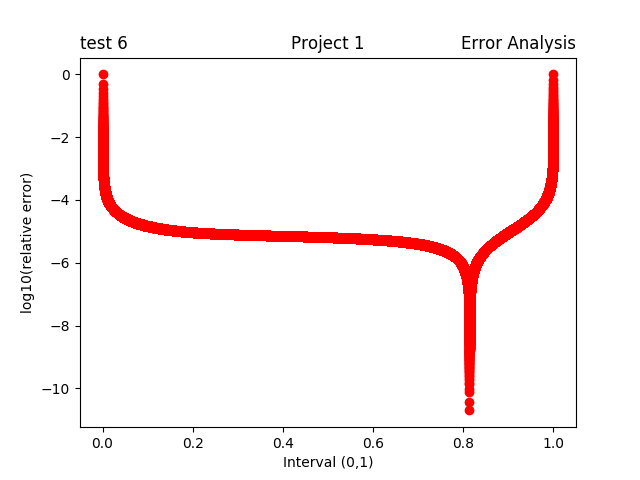
\includegraphics[width=\linewidth]{test_6.png}
  \caption{Step size of $10^{-6}$}
  \label{fig:Relative Error}
\end{figure}

\section{Conclusions and perspectives}
\section{C++ Code}
\begin{lstlisting}
#include <iostream>
#include <fstream>
#include <iomanip>
#include <cmath>
#include <vector>
#include <string>
#include <armadillo>


// use namespace for output and input
using namespace arma;
using namespace std;

// object for output files
ofstream ofile;

// Functions used
inline double f_actualInputSolution(double x){return 100.0*exp(-10.0*x);}
inline double exact(double x) {return 1.0-(1-exp(-10))*x-exp(-10*x);}

// Test function interface forward function declaration
void simpleTridiagonalAlg(int n,double *sol,double *x);
void generalTridiagonalAlg(int n,double *u,double *x,double *d,double *c,double *a);
\begin{listings}
// Begin main program
int main(int argc, char **argv)
{
    // The range of input exponent values and the current output filename variables
    int exponent    = 0;
    string filename;

    // We read also the basic name for the output file and the highest power of 10^n we want
    cout << "number of args: " << argc << endl;
    if( argc <= 1 )
    {
          cout << "Bad Usage: " << argv[0] <<
              " read also file name on same line and max power 10^n" << endl;
          exit(1);
    }
    else
    {
        // first command line argument after name of program
        filename    = argv[1];
        exponent    = atoi(argv[2]);
        cout << "Highest value of the exponent: " << exponent << endl;
    }

    double test = exact(1.0);
    cout << "test result: " << test << endl;

    // Loop over powers of 10
    for (int i = 1; i <= exponent; i++)
    {
      int n = (int) pow(10.0,i);

      // Declare new file name
      string fileout = filename;

      // Convert the power 10^i to a string
      string argument = to_string(i);

      // Final filename as filename-i-
      fileout.append(argument);

      // Dynamic array created for the diagonal, upper diagonal, and lower diagonal elemements
      double *d   = new double [n+1];
      double *c   = new double [n+1];
      double *a   = new double [n+1];

      //initialize with simple case of D problem
      for (int i=0; i < n+1; i++)
      {
          d[i]    = +2;
          a[i]    = -1;
          c[i]    = -1;
      }
      d[n]    = +2;

      // Set up the input grid, and solution array
      double *solution  = new double [n+1];
      double *x         = new double [n+1];

      // Test function interface
      // simpleTridiagonalAlg(n,solution,x);
      generalTridiagonalAlg(n,solution,x,d,a,c);

      // Make the current file
      ofile.open(fileout);
      ofile << setiosflags(ios::showpoint | ios::uppercase);

      //      ofile << "       x:             approx:          exact:       relative error" << endl;
      for (int i = 1; i < n + 1;i++)
      {
        double xval = x[i];
        double RelativeError = fabs((exact(xval)-solution[i])/exact(xval));
        ofile << setw(15) << setprecision(8) << xval;
        ofile << setw(15) << setprecision(8) << solution[i];
        ofile << setw(15) << setprecision(8) << exact(xval);
        ofile << setw(15) << setprecision(8) << log10(RelativeError) << endl;
      }
      ofile.close();

      // clean up for next interation
      delete [] x; delete [] solution; delete [] d;  delete [] a; delete [] c;
    }

    return 0;
}

// Program function definitions

// Simple case of the tri-diagonal algorithm
void simpleTridiagonalAlg(int n,double *sol,double *x)
{
    // Set up arrays for the simple case
    double *d = new double [n+1];
    double *b = new double [n+1];

    // Quick setup of updated diagonal elements and value of the simple verion of the tri-diagonal matrix
    double h    = 1.0/(n+1);
    double hh   = h*h;
    d[0]        = d[n]      = 2;
    sol[n]      = 0.0;
    for (int i = 0; i <= n; i++)
    {
      x[i]= i*h;
      b[i] = hh*f_actualInputSolution(i*h);
    }

    // Forward substitution
    for (int i = 1; i < n; i++)
    {
        d[i] = (i+1.0)/( (double) i);
    }

    for (int i = 1; i < n+1; i++)
    {
        b[i] = b[i] + b[i-1]/d[i-1];
    }

    // Backward substitution
    for (int i = n-1; i > 0; i--)
    {
        sol[i] = (b[i]+sol[i+1])/d[i];
    }
}

// General case if the tri-diagonal algoritm
void generalTridiagonalAlg(int n,double *u,double *x,double *d,double *c,double *a)
{
    // array of values of f in the nxn system
    double *v = new double [n+1];

    // Quick setup of updated diagonal elements and value of the general verion of the tri-diagonal matrix
    double h    = 1.0/(n+1);
    double hh   = h*h;
    for (int i = 0; i < n+1; i++)
    {
      x[i]= i*h;
      v[i] = hh*f_actualInputSolution(i*h);
    }

    // Forward substitution
    //modify the diagonal elements
    for (int i = 1; i < n+1; i++)
    {
        d[i] = d[i] - c[i-1]*a[i]/d[i-1];
    }

    //modify the desired output values for the system to correspond with the changes made by the Forward Substitution above
    for (int i = 1; i < n + 1; i++)
    {
        v[i] = v[i] - v[i-1]*a[i]/d[i-1];
    }

    // Backward substitution gives the final solution
    u[n] = v[n]/d[n];
    for (int i = n; i > 0; i--)
    {
        u[i-1] = (v[i] - c[i]*u[i])/d[i-1];
    }
}

\end{lstlisting}

\end{document}  